\section{Accurate analytical modeling for hydrostatic stress evolution}
\label{sec:multi_segment}
In this paper, an accurate analytical modeling for transient hydrostatic stress analysis for a general realistic interconnect structure as shown in Fig.\ref{fig:interconnect_tree}, which represents a long metal wire with a number of the voltage and current ports. Since many complex interconnect structures such as power grids could be decomposed to hierarchically in smaller interconnect components, the accurate analytic closed-form expressions describing hydrostatic stress evolution for multi-branch interconnect trees will lay the groundwork for the EM reliability analysis of complex interconnect networks. Based on the Laplace transformation technique, an accurate closed-form expression during the void nucleation phase for the long metal wire shown in Fig.\ref{fig:interconnect_tree} will be proposed.
\label{sec:analytical_stress}
\begin{figure}[ht] \centering
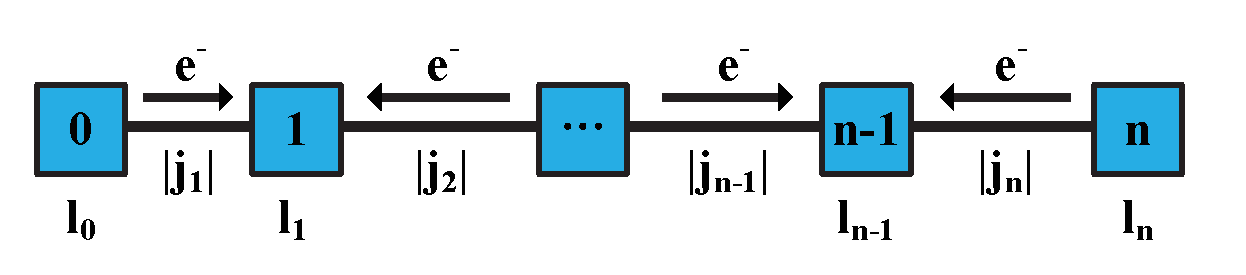
\includegraphics[width=80mm]{Sn.eps}
\caption{An example of general realistic interconnect structure.}
  \label{fig:interconnect_tree}
  \vspace{-0.12in}
\end{figure}

The stress evolution process for each segment in Fig.\ref{fig:interconnect_tree} is described by the Korhonen equation. Stress evolution equations for each segment are coupled to each other by the boundary conditions representing the continuity of stress and fluxes at the junctions in the long metal wire. The general system of equation in this case can be described as follows:
\begin{equation} \label{eq:general_interconnect_tree}
\begin{split}
&\frac{\partial \sigma_1}{\partial t}=\frac{\partial }{\partial
x}[\kappa_1(\frac{\partial \sigma_1}{\partial x}+G_1)],\;l_0\leq x \leq l_1 \\
&\frac{\partial \sigma_2}{\partial t}=\frac{\partial }{\partial
x}[\kappa_2(\frac{\partial \sigma_2}{\partial
x}+G_2)],\;l_1\leq x \leq l_2, \\
&\cdots\cdots\\
&\frac{\partial \sigma_{n-1}}{\partial t}=\frac{\partial }{\partial
x}[\kappa_{n-1}(\frac{\partial \sigma_{n-1}}{\partial
x}+G_{n-1})],\;l_{n-2}\leq x \leq l_{n-1}, \\
&\frac{\partial \sigma_{n}}{\partial t}=\frac{\partial }{\partial
x}[\kappa_{n}(\frac{\partial \sigma_{n}}{\partial
x}+G_{n})],\;l_{n-1}\leq x \leq l_n.
 \end{split}
 \end{equation}
In \eqref{eq:general_interconnect_tree}, $\kappa_{i}$ and $G_i$ ($i=1,2,\cdots,n$) are the stress diffusivity and the EM driving force for each segment wire.
Boundary conditions for these equations are given as the follows:
 \begin{equation} \label{bc:general_interconnect_tree}
\begin{split}
&\kappa_1(\frac{\partial \sigma_1}{\partial x}+G_1)=0,\;x=l_0,\\
&\sigma_1=\sigma_2,\;x=l_1,\\
&\kappa_1(\frac{\partial \sigma_1}{\partial
x}+G_1)=\kappa_2(\frac{\partial \sigma_2}{\partial
x}+G_2),\;x=l_1,\\
&\sigma_2=\sigma_3,\;x=l_2,\\
&\kappa_2(\frac{\partial \sigma_2}{\partial
x}+G_2)=\kappa_3(\frac{\partial \sigma_3}{\partial
x}+G_3),\;x=l_2,\\
&\cdots\cdots \\
&\kappa_n(\frac{\partial \sigma_n}{\partial
x}+G_n)=0,\;x=l_n.
 \end{split}
 \end{equation}
Initial conditions for the void nucleation phase are given by $\sigma_i=0$ at $t=0$ at each segment. The Laplace transformation technique can be used to obtain an accurate closed-form expression for the void stress evolution equations \eqref{eq:general_interconnect_tree}. For the sake of simplicity, we need to assume that $\kappa_1=\kappa_2=\cdots=\kappa_k$. After transforming \eqref{eq:general_interconnect_tree}-\eqref{bc:general_interconnect_tree} by the Laplace transformation technique, we get a system of ordinary differential equations (ODEs). In order to derive the solution of each ODE, we first need to introduce the following notations:
\begin{equation} \label{generalNotations}
\begin{split}
&\xi_{n,1}^{i}(m,x)=l_n+2m(l_n-l_0)-x,\\
&\xi_{n,2}^{i}(m,x)=(2l_n-l_0)+2m(l_n-l_0)-x,\\
&\xi_{n,2j+1}^{i}(m,x)=(2l_n-l_j)+2m(l_n-l_0)-x,\\
&\xi_{n,2j+2}^{i}(m,x)=\left\{
   \begin{aligned}
   &(2l_n-2l_0+l_j)+2m(l_n-l_0)-x,\;\\
   &\qquad\qquad\qquad\qquad\qquad\quad 0<j<i,  \\
   &l_j+2m(l_n-l_0)-x,\;i\leq j\leq n-1, \\
      \end{aligned}
   \right. \\
&\eta_{n,1}^{i}(m,x)=(l_n-2l_0)+2m(l_n-l_0)+x,\\
&\eta_{n,2}^{i}(m,x)=-l_0+2m(l_n-l_0)+x,\\
&\eta_{n,2j+1}^{i}(m,x)=(l_j-2l_0)+2m(l_n-l_0)+x,\\
&\eta_{n,2j+2}^{i}(m,x)=\left\{
   \begin{aligned}
   &-l_j+2m(l_n-l_0)+x,\;0<j<i,  \\
   &(2l_n-l_j-2l_0)+2m(l_n-l_0)+x,\; \\
   &\qquad\qquad\qquad\qquad\qquad i\leq j \leq n-1. \\
   \end{aligned}
   \right.
\end{split}
\end{equation}
Similar to the analytical method introduced in \cite{?}, we need to construct the following basic function:
\begin{equation} \label{general_basisFunc}
g(x,t)=2\sqrt{\frac{\kappa t}{\pi}}e^{-\frac{x^2}{4\kappa
t}}-x\times\texttt{erfc}\{\frac{x}{2\sqrt{\kappa t}}\}.
\end{equation}
where the complementary error function $\texttt{erfc}\{x\}$ is defined as $\texttt{erfc}\{x\}=\frac{2}{\sqrt{\pi}}\int_x^{+\infty}e^{-t^2}dt$. Thus, a general form of analytical solutions of stress evolution equations for all segments can be written as follows
\begin{equation} \label{eq:general_solution}
\begin{split}
\sigma_{n,i}&(x,t)=-\sum\limits_{m=0}^{+\infty}\{G_ng(\xi_{n,1}^{i},t)-G_1g(\xi_{n,2}^{i},t)\\
&-\sum\limits_{j=1}^{n-1}\frac{G_{j+1}-G_j}{2}(g(\xi_{n,2j+1}^{i},t)-g(\xi_{n,2j+2}^{i},t))\}\\
&-\sum\limits_{m=0}^{+\infty}\{G_ng(\eta_{n,1}^{i},t)-G_1g(\eta_{n,2}^{i},t)\\
&-\sum\limits_{j=1}^{n-1}\frac{G_{j+1}-G_j}{2}(g(\eta_{n,2j+1}^{i},t)-g(\eta_{n,2j+2}^{i},t))\}.
 \end{split}
 \end{equation}

In practical calculation, we should develop an approximate analytic formula of the exact series solution \eqref{eq:general_solution} for multi-segment interconnect wire. The approximate solution using the first dominant term for each segment in the interconnect wire provides
\begin{equation} \label{eq:approximate_solution}
\begin{split}
&\sigma_{n,i}(x,t)\approx-\{G_ng(\xi_{n,1}^{i}(0,x),t)-G_1g(\xi_{n,2}^{i}(0,x),t)\\
&-\sum\limits_{j=1}^{n-1}\frac{G_{j+1}-G_j}{2}(g(\xi_{n,2j+1}^{i},t)(0,x)-g(\xi_{n,2j+2}^{i}(0,x),t))\}\\
&-\{G_ng(\eta_{n,1}^{i}(0,x),t)-G_1g(\eta_{n,2}^{i}(0,x),t)\\
&-\sum\limits_{j=1}^{n-1}\frac{G_{j+1}-G_j}{2}(g(\eta_{n,2j+1}^{i}(0,x),t)-g(\eta_{n,2j+2}^{i}(0,x),t))\}.
 \end{split}
 \end{equation}
It should be noted that the present analysis method in analytical characterization is similar to what has been reported in our early work of analytical modeling of electromigration for multi-branch interconnect tree. However, the purpose of this paper is not to develop any new analysis method, but to illustrate the closed-form expression for the solution of stress evolution equations for more complex interconnect trees embedded in the frequently employed circuits. 


%After transforming all the equations and the corresponding BC into Laplace space we get a system of $n$ equations similar to \eqref{eq:dotted_I_tree_lap} and BC represented by $n+1$ equations similar to \eqref{bc:dotted_I_tree_lap}. Solution of each ODE represented by \eqref{eq:dotted_I_tree_fre} with two unknown parameters, which will be found from BC, similarly to what was done in the case of two-segments/three terminals case, \eqref{cofficients_I}. A problem that we are solving is determination of the moment of time and location on the $\mathrm{V_{DD}}$ rail when and where the first void will be nucleated. To do this we do not need to make the inverse Laplace transformation. It is enough to compare the stress in the Laplace space $\sigma_i(x,s)$ with the Laplace transform of the critical stress. It should be also taken into account that not all junctions but just some of them can provide a condition for void nucleation: $\sigma=\sigma_{crit}$. Basically just two types of junctions characterized by specific configurations of the current directions should be considered. First type is the terminating segments serving as the current outlets (electron cathodes), and second the junctions separating two segments with electron flows directed outward this junctions.




